\section{Intercepts, Zeros, Roots, Solutions and Factors}

\begin{myCenteredBox}[width=4in, colback=white, ]
    The following concepts are all very closely related:
    \begin{itemize}[nosep]
        \item {\bfseries\itshape $x$-intercepts} of a function, $f(x)$
        \item {\bfseries\itshape zeros} of a function, $f(x)$
        \item {\bfseries\itshape solutions} of the equation $f(x) = 0$
        \item {\bfseries\itshape roots} of the equation $f(x) = 0$
        \item the {\bfseries\itshape factors} of a function, $f(x)$
    \end{itemize}
    Given one, you can find the others.
\end{myCenteredBox}
The graph of 
{
    $f(x) = x^3 + x^2 -2x $
}
is shown below. 
The zeros, roots/solutions and factors are easy to find.
\begin{minipage}{0.3\textwidth}
\begin{center}
\begin{tikzpicture}[
    scale=0.5,
    xaxe style/.style = { very thick, arrows={-{Straight Barb}}, label={}, },                 
    yaxe style/.style = { very thick, arrows={-{Straight Barb}}, label={}, },                 
]
\scriptsize
\tkzInit[ xmax=4, xmin=-4,  ymax=4, ymin=-4, ]
\tkzGrid
\tkzDrawXY[label={},color=black,]
% \tkzLabelX[orig=false,]
% \tkzLabelY[orig=false,]
\tkzFct[domain = -4:4,thick, solid]{x*x*x + x*x - 2*x}
\tkzText[left](-1.5,2){\Large$f$}
\end{tikzpicture}
\end{center}
\end{minipage}
%
\begin{minipage}{0.69\textwidth}
    \begin{itemize}
        \item the {\bfseries\itshape $x$-intercepts} of $f$ are \gap{(-2,0)}, \gap{(0,0)},\\ and \gap{(1,0)}.
        \item the {\bfseries\itshape zeros} of $f$ are \gap{-2}, \gap{0}, and \gap{1}.
    \end{itemize}
    \begin{itemize}
        \item the {\bfseries\itshape factors} of $f$ are \gap{$(x+2)$}, \gap{$x$}, and \gap{$(x-1)$}.
        \item the {\bfseries\itshape roots/solutions} of the equation $f(x)=0$ are \gap{-2}, \gap{0},\\ and \gap{1}.
    \end{itemize}
\end{minipage}


\begin{taggedblock}{on-level}
    \begin{myProblemsWithContent}{1}{%
        \begin{itemize}[nosep]
            \item Sketch the graph of $y=f(x)$ using {\scshape Desmos}.
            \item Factor the given polynomial function, $f(x)$. 
            \item Solve the equation $f(x)=0$.
            \item Then fill in the blanks based on your results.
        \end{itemize}
        }
        {\large $f(x) = x^3 + 5x^2 + 6x$}
        \tcblower
    
        \begin{minipage}{0.3\textwidth}
            \begin{center}
            \begin{tikzpicture}[
                scale=0.55,
                xaxe style/.style = { very thick, arrows={-{Straight Barb}}, label={}, },                 
                yaxe style/.style = { very thick, arrows={-{Straight Barb}}, label={}, },                 
            ]
            \scriptsize
            \tkzInit[ xmax=4, xmin=-4,  ymax=4, ymin=-4, ]
            \tkzGrid
            \tkzDrawXY[label={},color=black,]
            % \tkzLabelX[orig=false,]
            % \tkzLabelY[orig=false,]
            % \tkzFct[domain = -4:4,thick, solid]{x**4 - 5*x**2 + 4}
            % \tkzText[left](-1.5,2){\Large$f$}
            \end{tikzpicture}
            \end{center}
        \end{minipage}
        
        \begin{itemize}
            \item $x$-intercepts:\quad \underline{\hspace{3in}}
            \item zeros:\quad \underline{\hspace{3in}}
            \item factors:\quad \underline{\hspace{3in}}
            \item roots/solutions:\quad \underline{\hspace{3in}}
        \end{itemize}
    \end{myProblemsWithContent}
\end{taggedblock}
    
\begin{taggedblock}{pre-AP}
\begin{myProblemsWithContent}{1}{%
    \begin{itemize}[nosep]
        \item Sketch the graph of $y=f(x)$ using {\scshape Desmos}.
        \item Factor the given polynomial function, $f(x)$. 
        \item Solve the equation $f(x)=0$.
        \item Then fill in the blanks based on your results.
    \end{itemize}
    }
    {\large $f(x) = x^4 - 5x^2 + 4$}
    \tcblower

    \begin{minipage}{0.3\textwidth}
        \begin{center}
        \begin{tikzpicture}[
            scale=0.55,
            xaxe style/.style = { very thick, arrows={-{Straight Barb}}, label={}, },                 
            yaxe style/.style = { very thick, arrows={-{Straight Barb}}, label={}, },                 
        ]
        \scriptsize
        \tkzInit[ xmax=4, xmin=-4,  ymax=4, ymin=-4, ]
        \tkzGrid
        \tkzDrawXY[label={},color=black,]
        % \tkzLabelX[orig=false,]
        % \tkzLabelY[orig=false,]
        % \tkzFct[domain = -4:4,thick, solid]{x**4 - 5*x**2 + 4}
        % \tkzText[left](-1.5,2){\Large$f$}
        \end{tikzpicture}
        \end{center}
    \end{minipage}
    
    \begin{itemize}
        \item $x$-intercepts:\quad \underline{\hspace{3in}}
        \item zeros:\quad \underline{\hspace{3in}}
        \item factors:\quad \underline{\hspace{3in}}
        \item roots/solutions:\quad \underline{\hspace{3in}}
    \end{itemize}
\end{myProblemsWithContent}
\end{taggedblock}




\begin{myProblemsWithContent}{1}{%
    Use the graph of the polynomial function $f(x)$ to find the zeros, roots, $x$-intercepts, and factors 
    of $f(x)$.
    }
    \begin{minipage}{0.3\textwidth}
        \begin{center}
        \begin{tikzpicture}[
            scale=0.55,
            xaxe style/.style = { very thick, arrows={-{Straight Barb}}, label={}, },                 
            yaxe style/.style = { very thick, arrows={-{Straight Barb}}, label={}, },                 
        ]
        \scriptsize
        \tkzInit[ xmax=4, xmin=-4,  ymax=4, ymin=-4, ]
        \tkzGrid
        \tkzDrawXY[label={},color=black,]
        % \tkzLabelX[orig=false,]
        % \tkzLabelY[orig=false,]
        \tkzFct[domain = -4:4,very thick, solid]{0.5*( (x+1)*(x-2)*(x-3))}
        \tkzText[left](-1,2){\Large$f$}
        \end{tikzpicture}
        \end{center}
    \end{minipage}

    \tcblower

    \begin{itemize}
        \item $x$-intercepts:\quad \underline{\hspace{3in}}
        \item zeros:\quad \underline{\hspace{3in}}
        \item factors:\quad \underline{\hspace{3in}}
        \item roots/solutions:\quad \underline{\hspace{3in}}
    \end{itemize}
\end{myProblemsWithContent}

\begin{taggedblock}{on-level}
    \begin{my2Problems}{3in}[Factor the given polynomial function to find its factors. Then find the roots/solutions of $f(x)=0$. ]
        {
            $f(x) = x^2 + 2x - 8$
        }
        {
            $f(x) = x^3 + 2x^2 - 9x - 18$
        }
\end{my2Problems}
\end{taggedblock}
\begin{taggedblock}{pre-AP}
    \begin{my2Problems}{3in}[Factor the given polynomial function to find its factors. Then find the roots/solutions of $f(x)=0$. ]
        {
            $f(x) = x^3 + 5x^2 - 16x - 80$
        }
        {
            $f(x) = x^3 + 2x^2 - 9x - 18$
        }
    \end{my2Problems}
\end{taggedblock}